The advent of effective digital video compression was key to the development of today’s multimedia systems.

Upon its invention in the 1970s \cite{ghanbari_2003}, digitized studio-quality video had \emph{enormous} bandwidth requirements, making it impractical to be transmitted over any telecommunications system.
In fact, those requirements would practically never be met until the 1990s \cite{wiki:Video_coding_format}.

The solution was then to find a way to \emph{compress} video data (most often along its audio counterpart in \emph{containers} \cite{wiki:Digital_container_format}) as efficiently as possible.
The newly engineered compression standards and transmission protocols -- stringed together -- made possible to stream higher-quality video over low-bandwidth networks.
Incrementally improving those techniques, as well as the increased availability of broadband connections today, has led to the widespread use of high-definition video on television and over the Internet, often at high speeds as well.

In this section, we present the evolution of digital video formats from the first practically viable technologies to the widespread adoption of Internet streaming platforms.

\section{DCT and Motion-compensated DCT}
\textbf{DCT compression} constitutes the core of all standard codecs \cite{ghanbari_2003}, and will subsequently lead to the development of the H.261 and MPEG encoding standards -- widely considered the \emph{first practical video formats} \cite{wiki:Timeline_of_online_video}.

DCT itself stands for \emph{Discrete Cosine Transform} and represents a technique for decomposing a signal into a set of cosine functions, each oscillating at a different frequency \cite{wiki:Discrete_cosine_transform}.
This process was first proposed by \textbf{Nasir Ahmed} in 1972 \cite{wiki:Discrete_cosine_transform}, who originally intended it for use in \emph{image compression} \cite{wiki:Video_coding_format}.
(Subsequently, the JPEG standard for compressing static images was developed to use this principle.)

\emph{DCT compression} is a type of lossy compression, also known as \emph{block compression}, due to compressing data in concrete blocks \cite{wiki:Discrete_cosine_transform}.
This type of compression, however, would not be practical enough for widespread application until the advent of motion-compensated DCT.

\textbf{Motion-compensated DCT} \cite{wiki:Video_coding_format} is a hybrid algorithm, since it combines two techniques. One of them is DCT, which is used for the spatial dimension.
The other key component is motion-compensated hybrid coding, used for the temporal dimension.

MC-DCT became the \emph{standard technique} for video compression from the late 1980s onwards \cite{wiki:Video_coding_format}.

\section{Modern Video: the H.26x and MPEG Families}
The development of \emph{motion-compensated DCT} would open up a myriad of directions for further development and adaptation of this new video compression technique.
One of the first significant leaps forward was \emph{H.261}.

In November 1988, the ITU-T
\footnote{\emph{ITU Telecommunication Standardization Sector (ITU-T)} is a specialized agency of the United Nations which coordinates standards for telecommunication and ICT \cite{wiki:ITU-T}}
released the H.261 compression standard \cite{wiki:H.261} which was based on motion-compensated DCT \cite{ghanbari_2003}.

\textbf{H.261} would be considered the first major video compression standard \cite{real_timeline}, after its predecessor -- H.120 -- failed to be of any practical use \cite{real_timeline}.
MPEG-1 followed in 1991 \cite{real_timeline}, developed by the \emph{Motion Picture Experts Group (MPEG)}, and was designed to compress VHS-quality video \cite{real_timeline}.

The \textbf{H.26x and MPEG} series of standards, despite sharing many technical aspects, have evolved for different purposes and are now largely independent \cite{ghanbari_2003}.
H.26x specifications are managed by the ITU-T with the purpose of being used in telecommunication, while the MPEG specifications address the problem of video storage, television broadcast and streaming over the Internet \cite{ghanbari_2003}.

The managing committees joined forces to produce \textbf{MPEG-2} and \textbf{H.262} in 1994 \cite{real_timeline}.
This raised the bar for quality standards as it offered better resolution and higher bit rates.
The codecs in this family became the norm for \emph{DVDs} and \emph{digital TV} \cite{real_timeline}.

The \textbf{MPEG-4} was originally released in 1999 \cite{real_timeline} and sparked a revolution in terms of quality and bitrate, as well as multiple spin-off proprietary standards such as DivX and Xvid \cite{real_timeline}.

\textbf{Advanced Video Coding (AVC)} (also known as H.264 / MPEG-4 AVC) was started in 2003 by the same JVT (\emph{Joint Video Team}, the name of the partnership between the ITU-T and the MPEG committees) \cite{wiki:Advanced_Video_Coding}.
AVC has become the most widespread video encoding in 2019 according to Bitmovin \cite{wiki:Video_coding_format}.

The latest generation of video compression standards is \textbf{HEVC (High Efficiency Video Coding)} -- AVC’s successor -- developed in 2003 \cite{wiki:Video_coding_format}.
The core ideas and technologies which made MPEG-1 possible are used in the latest standards today.
For instance, HEVC still uses DCT, despite introducing a slight modification to the core algorithm (it uses integer-DCT, which processes integer numbers instead of real numbers) \cite{wiki:High_Efficiency_Video_Coding}.

\begin{figure}[ht]
    \caption{A timeline of video coding standards, as given in \cite{ghanbari_2003}.}
    \centering
    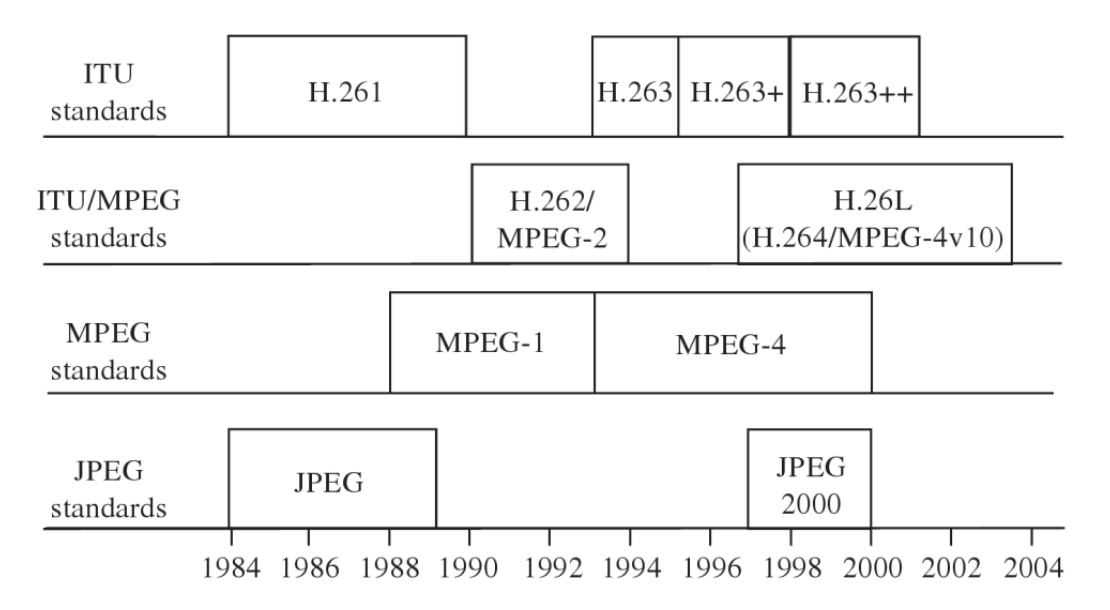
\includegraphics[width=\textwidth]{codec-timeline}
\end{figure}

\section{The Web and Mass-streaming Platforms}

The newly improved audio-video streaming technology empowers Internet users to communicate with colleagues at work as well as loved ones seamlessly over video chat and voice call with services such as \emph{Skype} and \emph{Zoom}.

Moreover, accesible and performant video technologies stand at the very foundation of many Internet empires such as \emph{YouTube} and \emph{Netflix}, as well as -- naturally -- playing an important role in social media, especially on platforms such as \emph{Snap} and \emph{Instagram} which are based on users creating and consuming short-form video content (sometimes called \emph{stories} or \emph{snaps} on their respective platforms).

Because the success stories are numerous, we will choose to present \emph{only one platform} (as a case study) that the author considers particularly important to the development of the modern Web.
In the following section we will outline a short history and explain why video compression played a major role in its development.

\subsection{YouTube: A Case Study}
\textbf{YouTube} is an online video-sharing platform founded in 2005 by former PayPal employees, later acquired by Google (in November 2006) as one of its subsidiaries \cite{wiki:YouTube}.

YouTube redefined the way people watch, produce and upload video content online.

The core mechanic of YouTube are \emph{channels}, allowing users to put up content and grow a fanbase through subscriptions.
This tool is as simple as it is powerful.

Boasting a solid userbase, its revenue is mostly obtained from running ad campaings to sustain the free service.
YouTube has also created a paid subscription-based model through YouTube Premium.

During its many years of operation, YouTube gave rise to many trends by making video blogging accesible to a wide audience.
It has content geared towards most age groups, on topics ranging from lifestyle to science and technology.
It is often credited for the popularization (if not creation) of the genre of \emph{Let's Play} and \emph{video game commentary} videos.

For many of the younger generations, YouTube has become the primary source of video content \cite{youtube_phrasee}.
This nudged traditional media towards implementing their own on-demand streaming services \cite{youtube_phrasee}.

On a more technical note, YouTube is an engineering marvel: supporting livestreams, serving video with near world-wide span reliably and with almost no downtime.
Part of what made YouTube possible is one of the aformentioned video codecs \emph{H.264}, which is the most commonly used compression on the platform \cite{youtube_quality}.
Other codecs are used as well, such as the Google-developed \emph{VP8} \cite{youtube_quality}, which is open and royalty-free \cite{wiki:VP8}.

